%% ============================================================
%%  Capitolo 1 – Introduzione alla Patologia Digitale
%%  Dispensa del Corso di Patologia Post-Laurea
%%  Questo file è incluso con \input{} da main.tex; NON aggiungere il preambolo qui.
%% ============================================================

\chapter{Introduzione alla Patologia Digitale}
\label{ch:1}

\section{Introduzione}

Per oltre un secolo e mezzo, la diagnosi istopatologica si è fondata su una tecnologia di apparente semplicità: una sottile sezione di tessuto, fissata chimicamente, inclusa in paraffina, colorata con ematossilina ed eosina (H\&E) o con un pannello di colorazioni speciali, e montata sotto un vetrino coprioggetto. Il vetrino così ottenuto viene esaminato al microscopio ottico in campo chiaro, e l'occhio esperto del patologo interpreta l'architettura cellulare, la morfologia nucleare e l'organizzazione tissutale per giungere a una diagnosi. Questo flusso di lavoro ha servito la medicina in modo straordinario, eppure presenta limitazioni intrinseche: i vetrini sono oggetti fisici fragili che si deteriorano nel tempo, i microscopi sono vincolati a una singola postazione, i secondi pareri richiedono il trasporto fisico di materiale insostituibile, e la natura soggettiva e analogica della valutazione visiva rende difficile conseguire una riproducibilità quantitativa.

L'affermarsi della \emph{patologia digitale} nel corso degli ultimi due decenni rappresenta la trasformazione più significativa dell'istopatologia diagnostica dall'introduzione dell'immunoistochimica. Nella sua essenza, la patologia digitale sostituisce il microscopio ottico, quale strumento primario di osservazione, con un'immagine digitale ad alta risoluzione dell'intero vetrino --- una \emph{whole slide image} (WSI) --- che può essere archiviata, trasmessa, visualizzata e analizzata computazionalmente. Questo cambiamento non è una mera comodità tecnologica: modifica in modo fondamentale ciò che è possibile nella pratica patologica, nella didattica, nella ricerca e nella garanzia della qualità. La refertazione a distanza, i tumor board multisede, la ricerca su larga scala di biomarcatori e la diagnosi assistita dall'intelligenza artificiale dipendono tutti dall'immagine digitale come tipo di dato fondamentale \cite{bera2019}.

Il ritmo di adozione si è accelerato notevolmente da quando gli enti regolatori di diverse giurisdizioni hanno concesso l'approvazione per la diagnosi primaria mediante WSI. Nel Regno Unito, il programma di trasformazione della patologia di NHS England ha identificato la patologia digitale come priorità strategica, e molti centri medici accademici gestiscono oggi servizi diagnostici completamente o parzialmente digitali. A livello internazionale, la convergenza tra scanner ad alto rendimento a costi accessibili, infrastrutture di archiviazione cloud e software di analisi delle immagini validati ha abbassato le barriere all'adozione per istituzioni di ogni dimensione \cite{song2023}.

Il presente capitolo fornisce le basi concettuali e pratiche utili per  affrontare gli argomenti più avanzati trattati nei capitoli successivi. Prende avvio dalla definizione di patologia digitale e dalla sua collocazione nel più ampio panorama della patologia computazionale. Esamina quindi in dettaglio la tecnologia del whole slide imaging, trattando l'hardware degli scanner, i formati delle immagini, i concetti di risoluzione e i metadati. Il capitolo affronta poi le modalità di integrazione dei sistemi di patologia digitale con i sistemi informativi di laboratorio e l'infrastruttura informatica ospedaliera, per poi concentrarsi sulle responsabilità specifiche del tecnico di laboratorio biomedico nel flusso di lavoro digitale. Due attività pratiche strutturate consolidano i contenuti teorici, e il capitolo si chiude con un riepilogo e una serie di domande di verifica.

\section{Che cos'è la Patologia Digitale?}

La patologia digitale può essere definita come l'acquisizione, la gestione, la condivisione e l'interpretazione di informazioni patologiche --- incluse immagini, annotazioni e dati clinici associati --- in formato digitale. Nel senso più ristretto, il termine si riferisce alla digitalizzazione dei vetrini istologici per produrre whole slide images; nel senso più ampio, comprende l'intero ecosistema informatico che circonda tali immagini, dai sistemi informativi di laboratorio e dalle piattaforme di gestione delle immagini agli algoritmi di intelligenza artificiale e alle reti di telepatologia. Il Royal College of Pathologists e gli organismi equivalenti in Nord America e in Europa hanno adottato definizioni che sottolineano sia la dimensione tecnologica sia quella clinica: la patologia digitale non riguarda semplicemente il possesso di immagini digitali, ma l'utilizzo di tali immagini a supporto della diagnosi, della didattica, della ricerca e del miglioramento della qualità \cite{bankhead2022}.

È importante distinguere la patologia digitale dal campo correlato ma distinto della \emph{patologia computazionale}. La patologia digitale è la disciplina più ampia, che comprende tutti gli aspetti del lavoro con le immagini digitali di vetrini, indipendentemente dal fatto che sia coinvolta l'elaborazione computazionale. La patologia computazionale è una sotto-disciplina che applica metodi computazionali quantitativi --- analisi statistica delle immagini, apprendimento automatico, apprendimento profondo --- per estrarre informazioni da tali immagini che sarebbero difficili o impossibili da ottenere mediante la sola ispezione visiva \cite{campanella2019}. Un patologo che esamina una WSI su schermo pratica la patologia digitale; un modello di apprendimento profondo addestrato a rilevare figure mitotiche nella stessa immagine è un esempio di patologia computazionale. I due campi sono profondamente intrecciati e la distinzione è talvolta sfumata nella letteratura, ma è concettualmente utile mantenerla.

L'ambito della patologia digitale si estende a tutte le sottodiscipline dell'istopatologia e della citopatologia. La patologia chirurgica, la neuropatologia, la dermatopatologia, l'ematopatologia e la citologia hanno tutte sviluppato flussi di lavoro digitali, ciascuno con requisiti tecnici specifici. Le tecniche basate sulla fluorescenza, tra cui l'immunofluorescenza e l'ibridazione fluorescente in situ (FISH), richiedono scanner in grado di acquisire più canali di fluorescenza, aggiungendo complessità sia all'acquisizione sia all'archiviazione. I campioni citologici, spesso preparati come preparati in fase liquida su vetrini di grande formato, presentano sfide di scansione diverse rispetto alle sezioni istologiche standard. La diversità dei tipi di campione implica che una singola soluzione tecnica raramente soddisfi tutte le esigenze, e i tecnici di laboratorio biomedico devono comprendere i requisiti specifici di ciascuna modalità.

La patologia digitale si interseca inoltre con la \emph{telepatologia}, ovvero la pratica di trasmettere immagini patologiche attraverso una rete per consulenza o diagnosi a distanza. La telepatologia precede la moderna WSI --- i primi sistemi utilizzavano microscopi robotici controllati via linea telefonica --- ma la WSI l'ha trasformata in un servizio pratico e scalabile. La telepatologia per sezioni al congelatore, in cui una WSI di una sezione intraoperatoria viene trasmessa a un patologo remoto per una diagnosi immediata, è oggi in uso clinico routinario presso molte istituzioni. La pandemia di COVID-19 ha accelerato l'adozione dei flussi di lavoro di refertazione a distanza, dimostrando che la diagnosi primaria di alta qualità da WSI è fattibile e sicura quando sono in atto adeguate misure di garanzia della qualità \cite{song2023,giaretto2021}.

\section{Whole Slide Imaging: Principi e Strumenti}

\subsection{Funzionamento degli Scanner per Vetrini Interi}

Uno scanner per vetrini interi è, nella sua essenza, un microscopio automatizzato accoppiato a una fotocamera digitale ad alta risoluzione e controllato da un software che acquisisce sistematicamente l'intera superficie di un vetrino. La sfida fondamentale è di natura dimensionale: una sezione istologica standard può misurare $15 \times 10$\,mm o più, eppure le informazioni diagnostiche significative esistono a livello cellulare e subcellulare, richiedendo una risoluzione ottica di circa $0{,}25$\,\textmu m per pixel a ingrandimento $40\times$. Acquisire queste informazioni in una singola esposizione non è fattibile con la tecnologia di sensori attuale; gli scanner acquisiscono pertanto un gran numero di tessere (tile) di immagine sovrapposte o adiacenti e le uniscono computazionalmente per formare la WSI finale.

Il percorso ottico di uno scanner in campo chiaro è molto simile a quello di un microscopio convenzionale a luce trasmessa. La luce bianca proveniente da una sorgente LED o alogena attraversa un condensatore, poi la sezione di tessuto colorata, e infine entra nell'obiettivo. L'obiettivo proietta un'immagine ingrandita su una fotocamera a scansione lineare (negli scanner a scorrimento lineare) o su una fotocamera ad area (negli scanner a tessere). I sistemi a scansione lineare spostano il vetrino in modo continuo sotto una fotocamera fissa, acquisendo una striscia di dati immagine alla volta; i sistemi a tessere spostano il vetrino secondo uno schema a griglia, acquisendo campi visivi discreti. Entrambi gli approcci producono una qualità d'immagine equivalente se correttamente calibrati, ma differiscono nelle caratteristiche di throughput e nella suscettibilità agli artefatti da movimento.

La \emph{scansione in fluorescenza} segue gli stessi principi geometrici, ma sostituisce la sorgente di luce bianca trasmessa con una o più sorgenti di luce di eccitazione --- tipicamente LED ad alta potenza o linee laser --- e inserisce nel percorso ottico appropriati filtri di eccitazione ed emissione. Poiché l'emissione di fluorescenza è di ordini di grandezza più debole rispetto alla trasmissione in campo chiaro, gli scanner a fluorescenza richiedono fotocamere più sensibili (spesso sensori CMOS scientifici raffreddati o CCD), tempi di esposizione più lunghi e un'attenta gestione del fotosbiancamento. La WSI a fluorescenza multicanale, in cui lo stesso vetrino viene acquisito sequenzialmente attraverso più set di filtri, produce uno stack di immagini co-registrate che possono essere unite in un'immagine composita o analizzate canale per canale. Questa capacità è essenziale per i pannelli di immunofluorescenza multiplexata, sempre più utilizzati nella ricerca traslazionale e, più recentemente, nella diagnostica clinica \cite{bera2019}.

\subsection{Risoluzione e Ingrandimento}

La risoluzione di una WSI è determinata principalmente dall'apertura numerica (NA) dell'obiettivo e dalle dimensioni dei pixel del sensore della fotocamera. In pratica, gli scanner sono caratterizzati dall'ingrandimento ottico equivalente del loro obiettivo: gli obiettivi $20\times$ producono una dimensione del pixel di circa $0{,}50$\,\textmu m, mentre gli obiettivi $40\times$ producono circa $0{,}25$\,\textmu m per pixel. La scelta dell'ingrandimento di scansione comporta un compromesso tra il dettaglio dell'immagine e le dimensioni del file. Per la diagnosi routinaria con H\&E, la scansione a $20\times$ è generalmente considerata sufficiente; per le applicazioni che richiedono un fine dettaglio nucleare, il conteggio delle figure mitotiche o la localizzazione subcellulare dei marcatori immunoistochimici, è preferita la scansione a $40\times$. Alcuni scanner offrono un obiettivo a immersione in olio $60\times$ o $100\times$ per applicazioni specialistiche come l'ematologia o la microbiologia.

Le dimensioni dei file risultanti sono considerevoli. Una singola WSI a $20\times$ di una sezione tissutale standard occupa tipicamente da 500\,MB a 2\,GB di dati non compressi; a $40\times$, questo valore quadruplica. La compressione senza perdita o quasi senza perdita (JPEG\,2000, LZW) riduce i requisiti di archiviazione di un fattore da tre a cinque, ma anche i file compressi superano routinariamente i 500\,MB. Un laboratorio diagnostico impegnato che scansiona 200 vetrini al giorno genera oltre 100\,GB di nuovi dati immagine quotidianamente, ponendo richieste significative sull'infrastruttura di archiviazione, sulla larghezza di banda della rete e sui sistemi di archiviazione a lungo termine. Questi vincoli tecnici non sono preoccupazioni periferiche per il tecnico di laboratorio biomedico: influenzano direttamente la progettazione del flusso di lavoro, i protocolli di garanzia della qualità e la scelta della piattaforma di gestione delle immagini.

\subsection{Principali Produttori di Scanner}

Il mercato commerciale degli scanner WSI è dominato da un ristretto numero di produttori, ciascuno dei quali offre strumenti con caratteristiche tecniche, ecosistemi software e formati di file proprietari distinti.

\textbf{Aperio (Leica Biosystems)} produce le serie di scanner ScanScope e GT, che utilizzano un design ottico a scansione lineare e producono immagini nel formato SVS (ScanScope Virtual Slide). Gli scanner Aperio sono stati ampiamente impiegati sia in ambito clinico sia in quello della ricerca e sono stati tra i primi a ricevere l'autorizzazione regolatoria per la diagnosi primaria negli Stati Uniti. Il visualizzatore Aperio ImageScope e la piattaforma eSlide Manager sono comunemente presenti nei laboratori clinici.

\textbf{Hamamatsu Photonics} produce la serie NanoZoomer, che utilizza una fotocamera a scansione lineare con integrazione a ritardo di tempo (TDI) e produce immagini nel formato NDPI (NanoZoomer Digital Pathology Image). Gli scanner Hamamatsu sono particolarmente diffusi nei centri accademici giapponesi ed europei e sono noti per l'elevato throughput e la qualità costante delle immagini.

\textbf{Philips Digital Pathology} (ora parte di Philips Ultrasound \& Image Guided Therapy) produce la soluzione IntelliSite Pathology Solution, che utilizza un approccio di scansione a tessere e produce immagini nel formato iSyntax. Il sistema Philips è stata la prima piattaforma WSI a ricevere la marcatura CE per la diagnosi primaria in Europa ed è stata oggetto di diversi ampi studi di validazione clinica.

\textbf{3DHISTECH} (Budapest, Ungheria) produce la serie Pannoramic di scanner, che producono immagini nel formato MRXS. Gli strumenti 3DHISTECH sono ampiamente utilizzati in ambito di ricerca e didattico e offrono una gamma di opzioni di throughput, dai sistemi a vetrino singolo ai sistemi a carosello ad alta capacità.

\subsection{Software Open-Source per la Visualizzazione e l'Analisi}

Accanto alle piattaforme commerciali, si è sviluppato un vivace ecosistema di software open-source a supporto della visualizzazione, dell'annotazione e dell'analisi delle WSI. Due strumenti rivestono particolare importanza per il tecnico di laboratorio biomedico e il ricercatore in patologia.

\textbf{QuPath} (Quantitative Pathology \& Bioimage Analysis) è un'applicazione multipiattaforma basata su Java, sviluppata presso la Queen's University Belfast e successivamente presso l'Università di Edimburgo \cite{bankhead2017}. QuPath fornisce un visualizzatore WSI completo con supporto per tutti i principali formati proprietari (tramite la libreria OpenSlide), insieme a un'ampia suite di strumenti di analisi delle immagini che include il rilevamento cellulare, la classificazione tissutale, la quantificazione della fluorescenza e la programmazione tramite un'API basata su Groovy. La combinazione di accessibilità, estensibilità e rigore statistico ne ha fatto lo strumento open-source più utilizzato nella ricerca in patologia digitale \cite{bankhead2022}. QuPath è disponibile gratuitamente all'indirizzo \url{https://qupath.github.io} ed è attivamente mantenuto con rilasci regolari.

\textbf{OpenSlide} è una libreria C (con binding per Python, Java e altri linguaggi) che fornisce un'interfaccia di programmazione unificata per la lettura di file WSI in più formati proprietari, tra cui SVS, NDPI, MRXS, SCN e altri. Sviluppata presso la Carnegie Mellon University, OpenSlide astrae i dettagli specifici del formato della struttura dei file di ciascun produttore, consentendo agli sviluppatori di scrivere codice di analisi delle immagini che funziona su diverse piattaforme di scanner senza modifiche. È una dipendenza fondamentale di QuPath e di molti altri strumenti open-source, e la comprensione delle sue capacità e limitazioni è importante per chiunque sviluppi pipeline di analisi personalizzate.

\section{Formati delle Immagini Digitali, Risoluzione e Metadati}

\subsection{Struttura dei Pixel e Rappresentazione del Colore}

Al livello più fondamentale, un'immagine digitale è un array rettangolare di \emph{pixel} (elementi immagine), ciascuno dei quali memorizza un valore numerico che rappresenta il colore o l'intensità della luce in quella posizione. Nell'istologia standard in campo chiaro, le immagini vengono acquisite nel modello di colore RGB: ogni pixel è rappresentato da tre valori interi a 8 bit, uno per ciascuno dei canali di colore rosso, verde e blu, con ogni valore compreso tra 0 (nessun contributo da quel canale) e 255 (contributo massimo). La combinazione dei tre valori di canale definisce un colore da una tavolozza di $256^3 = 16{,}777{,}216$ colori possibili, sufficiente a rappresentare l'intera gamma di colori riscontrati nell'H\&E e nella maggior parte delle colorazioni speciali.

La convenzione degli 8 bit per canale è profondamente radicata nell'ecosistema WSI e nelle librerie di elaborazione delle immagini che operano sui dati WSI. È tuttavia importante essere consapevoli dei suoi limiti. Le immagini a fluorescenza, in particolare quelle acquisite con fotocamere di livello scientifico, vengono spesso acquisite a una profondità di 12 o 16 bit per canale, fornendo rispettivamente 4.096 o 65.536 livelli di intensità. Questo maggiore intervallo dinamico è importante per le misurazioni quantitative della fluorescenza, in cui deve essere preservata la relazione tra l'intensità del pixel e la concentrazione del fluoroforo. Quando le immagini a fluorescenza a 16 bit vengono convertite a 8 bit per la visualizzazione o l'archiviazione, le informazioni vengono irrimediabilmente perse a meno che la conversione non venga eseguita con attenzione e con un'appropriata scalatura. I tecnici di laboratorio biomedico coinvolti nella scansione a fluorescenza devono comprendere questa distinzione e assicurarsi che le pipeline di analisi operino alla profondità di bit appropriata.

\subsection{Piramidi di Immagini e Formati a Tessere}

Una WSI non può essere caricata interamente in memoria su una workstation standard; una scansione a $40\times$ di un grande campione di resezione può contenere $100{,}000 \times 80{,}000$ pixel o più, richiedendo diversi gigabyte di RAM per essere mantenuta non compressa. Per consentire una navigazione e una visualizzazione efficienti a più livelli di zoom, i file WSI vengono archiviati come \emph{piramidi di immagini}: una serie di versioni progressivamente sottocampionate dell'immagine a piena risoluzione, ciascuna con la metà della risoluzione lineare del livello precedente. Un'applicazione di visualizzazione carica solo il livello della piramide appropriato al fattore di zoom corrente e, all'interno di quel livello, solo le tessere che rientrano nel viewport corrente. Questa architettura consente una navigazione fluida e reattiva di immagini gigapixel su hardware con memoria limitata.

La piramide di immagini è tipicamente archiviata in un formato \emph{a tessere}, in cui ogni livello della piramide è suddiviso in una griglia regolare di piccole tessere (comunemente $256 \times 256$ o $512 \times 512$ pixel), ciascuna compressa in modo indipendente. La compressione indipendente delle tessere consente a un visualizzatore di decomprimere e visualizzare una singola tessera senza leggere l'intero file, riducendo drasticamente l'overhead di I/O, ovvero il tempo, i cicli della CPU e la memoria che viene utilizzata in operazioni di input/output che non contribuiscono al raggiungimento dell'operazione. I principali formati WSI proprietari --- SVS (Aperio), NDPI (Hamamatsu), MRXS (3DHISTECH) e iSyntax (Philips) --- implementano tutti varianti di questa architettura a piramide di tessere, sebbene differiscano nei loro specifici schemi di compressione, nelle dimensioni delle tessere e nelle strutture dei contenitori di file.

\textbf{OME-TIFF} (Open Microscopy Environment Tagged Image File Format) è un formato aperto e indipendente dal produttore che ha acquisito una posizione di rilievo come standard per lo scambio di WSI. OME-TIFF archivia i dati immagine in un contenitore TIFF standard con un blocco di metadati XML strutturato che codifica informazioni sulle dimensioni dell'immagine, le identità dei canali, le dimensioni fisiche dei pixel e i parametri di acquisizione in un vocabolario standardizzato. La variante BigTIFF di OME-TIFF supporta file di dimensioni superiori a 4\,GB, il che è essenziale per le WSI. L'adozione di OME-TIFF come formato di scambio comune è incoraggiata dagli enti regolatori e dalle organizzazioni di standardizzazione come mezzo per ridurre la dipendenza dai produttori e migliorare l'accessibilità dei dati a lungo termine \cite{song2023}.

\subsection{Concetti di Risoluzione: Micron per Pixel}

La risoluzione fisica di una WSI è espressa in \emph{micron per pixel} (\textmu m/px), che mette in relazione le dimensioni in pixel dell'immagine con le dimensioni fisiche del tessuto. Una scansione a $20\times$ ha tipicamente una risoluzione di circa $0{,}50$\,\textmu m/px, il che significa che ogni pixel corrisponde a un quadrato di tessuto di $0{,}5 \times 0{,}5$\,\textmu m. A $40\times$, questo valore si dimezza a circa $0{,}25$\,\textmu m/px. Il valore dei micron per pixel è memorizzato nei metadati dell'immagine ed è essenziale per qualsiasi misurazione quantitativa: le aree cellulari, i diametri nucleari, le distanze intercellulari e le dimensioni delle ghiandole sono tutti privi di significato senza la conoscenza della scala fisica.

È importante distinguere tra \emph{risoluzione ottica} (la caratteristica più piccola che l'obiettivo può risolvere, determinata dal criterio di Rayleigh e dalla NA dell'obiettivo) e \emph{risoluzione di campionamento digitale} (la dimensione del pixel). La teoria del campionamento di Nyquist richiede che la dimensione del pixel non sia superiore alla metà del limite di risoluzione ottica per evitare artefatti di aliasing. In pratica, la maggior parte degli scanner WSI è progettata in modo che la dimensione del pixel sia leggermente inferiore al limite di risoluzione ottica, garantendo che l'immagine digitale rappresenti fedelmente tutte le informazioni che l'ottica è in grado di acquisire. Il sovracampionamento oltre questo punto aumenta le dimensioni del file senza migliorare il contenuto informativo diagnostico.

\subsection{Metadati Incorporati nei File WSI}

I file WSI contengono ricchi metadati oltre ai dati pixel stessi. Questi metadati includono tipicamente: il modello e il numero di serie dello scanner; la data e l'ora di acquisizione; l'ingrandimento dell'obiettivo e l'apertura numerica; la dimensione fisica del pixel in micron; l'algoritmo di compressione e le impostazioni di qualità; l'immagine dell'etichetta del vetrino (una fotografia a bassa risoluzione dell'etichetta del vetrino di vetro); e, in alcuni formati, un'immagine macro che mostra l'intero vetrino a risoluzione molto bassa per scopi di navigazione. Nelle scansioni a fluorescenza, i metadati includono inoltre le lunghezze d'onda di eccitazione ed emissione per ciascun canale, i tempi di esposizione e le impostazioni di guadagno.

L'integrità dei metadati è fondamentale sia per le applicazioni cliniche sia per quelle di ricerca. In un contesto clinico, i metadati dello scanner forniscono una traccia di audit che collega l'immagine digitale al vetrino fisico e alla cartella del paziente. In un contesto di ricerca, i metadati consentono la riproducibilità: un ricercatore che analizza una coorte di WSI deve essere in grado di verificare che tutte le immagini siano state acquisite in condizioni comparabili. I tecnici di laboratorio biomedico responsabili della scansione devono pertanto assicurarsi che i registri di calibrazione dello scanner siano mantenuti, che le etichette dei vetrini siano correttamente associate agli identificativi del paziente prima della scansione e che tutti i campi di metadati richiesti dal sistema di gestione della qualità del laboratorio siano correttamente compilati. Gli errori nei metadati --- in particolare le discordanze degli identificativi del paziente --- costituiscono un grave rischio per la sicurezza del paziente e devono essere trattati con lo stesso rigore di qualsiasi altro errore pre-analitico in laboratorio.

\section{Integrazione con i Sistemi Informativi di Laboratorio}

\subsection{Sistemi Informativi di Laboratorio e LIMS}

Un \emph{Sistema Informativo di Laboratorio} (in inglese Laboratory Information System, LIS) è la piattaforma software che gestisce i dati amministrativi e clinici associati ai campioni patologici durante il loro ciclo di vita in laboratorio. Il LIS riceve le richieste dai team clinici (elettronicamente tramite sistemi di inserimento degli ordini o, in alcuni contesti, su moduli di richiesta cartacei), assegna numeri di accettazione univoci ai campioni, ne traccia il progresso attraverso il flusso di lavoro di laboratorio, archivia il referto del patologo e trasmette il referto finale al clinico richiedente. In un laboratorio di istopatologia, il LIS è il registro autorevole di ogni campione: collega i dati demografici del paziente, la storia clinica, la descrizione macroscopica, gli identificativi di blocco e livello, le richieste di colorazione e il referto diagnostico in un unico registro di caso coerente.

Un \emph{Laboratory Information Management System} (LIMS) è un concetto correlato ma distinto, più comunemente utilizzato in ambito di ricerca e industriale, che enfatizza il tracciamento dei campioni, la catena di custodia e la gestione dei dati piuttosto che la refertazione clinica. In pratica, i termini LIS e LIMS vengono talvolta usati in modo intercambiabile nella letteratura patologica, e molte piattaforme moderne sfumano la distinzione combinando funzionalità di refertazione clinica con capacità di gestione dei dati di ricerca. Ai fini del presente capitolo, il termine LIS verrà utilizzato per riferirsi al sistema di laboratorio clinico.

L'integrazione della patologia digitale con il LIS è un prerequisito per un'operatività clinica sicura ed efficiente. Quando un vetrino di vetro viene scansionato, la WSI risultante deve essere collegata in modo inequivocabile al caso corretto nel LIS. Questo collegamento viene tipicamente realizzato codificando il numero di accettazione del LIS e l'identificativo di blocco/livello in un codice a barre sull'etichetta del vetrino, che lo scanner legge automaticamente all'inizio di ogni scansione. Il software dello scanner trasmette quindi questo identificativo al sistema di gestione delle immagini (talvolta denominato sistema di gestione della patologia digitale o DPMS), che crea un record che collega il file WSI al caso nel LIS. Il patologo, quando apre un caso per la refertazione, visualizza la WSI insieme alle informazioni cliniche del LIS in un visualizzatore integrato, senza dover navigare tra sistemi separati.

\subsection{DICOM per la Patologia}

\emph{DICOM} (Digital Imaging and Communications in Medicine) è lo standard internazionale per l'archiviazione e la trasmissione di immagini mediche e delle informazioni associate. Originariamente sviluppato per la radiologia, DICOM è stato esteso alla patologia attraverso il Supplemento 145 (Whole Slide Microscopy Image) e i supplementi successivi. DICOM per la patologia definisce un formato di file standardizzato per i dati WSI che codifica sia i dati pixel (in una struttura a piramide di tessere) sia un insieme completo di attributi di metadati in un dizionario di dati standardizzato, inclusi i dati demografici del paziente, gli identificativi del campione, le informazioni sulla colorazione e i parametri di acquisizione.

L'adozione di DICOM come formato standard per le WSI cliniche offre diversi vantaggi importanti. In primo luogo, consente l'interoperabilità tra sistemi di produttori diversi: una WSI conforme a DICOM prodotta da uno scanner può, in linea di principio, essere visualizzata e refertata utilizzando qualsiasi visualizzatore conforme a DICOM, senza necessità di conversione del formato. In secondo luogo, si integra naturalmente con l'infrastruttura DICOM esistente dei reparti di radiologia ospedaliera, inclusi i PACS (Picture Archiving and Communication Systems) e i VNA (Vendor Neutral Archives), consentendo potenzialmente l'archiviazione e la gestione delle immagini patologiche all'interno della stessa piattaforma di imaging aziendale delle immagini radiologiche. In terzo luogo, i meccanismi maturi di sicurezza e traccia di audit di DICOM supportano i requisiti di governance della pratica clinica \cite{song2023}.

\subsection{Standard HL7 e Integrazione con l'Informatica Ospedaliera}

\emph{HL7} (Health Level Seven) è un insieme di standard internazionali per lo scambio di informazioni sanitarie cliniche e amministrative tra applicazioni software. La messaggistica HL7 versione 2 (HL7v2) è lo standard più ampiamente impiegato per l'integrazione del LIS negli ambienti informatici ospedalieri esistenti: i messaggi di ordine elettronico (ORM) vengono inviati dal sistema di inserimento degli ordini dell'ospedale al LIS quando viene richiesto un campione, e i messaggi di risultato (ORU) vengono inviati dal LIS al sistema clinico quando un referto viene autorizzato. HL7 FHIR (Fast Healthcare Interoperability Resources) è uno standard più recente basato su servizi web, sempre più adottato per le nuove integrazioni, in particolare nelle applicazioni sanitarie cloud e mobili.

Per la patologia digitale, la messaggistica HL7 fornisce il meccanismo attraverso il quale le informazioni sul campione e sul paziente fluiscono dai sistemi amministrativi dell'ospedale nel LIS e, da lì, nel sistema di gestione della patologia digitale. Un'interfaccia HL7 correttamente configurata garantisce che, quando un campione arriva in laboratorio, i dati demografici del paziente e le informazioni cliniche associate siano già presenti nel LIS, riducendo il rischio di errori di trascrizione. Consente inoltre la trasmissione automatica dei referti patologici alla cartella clinica elettronica del clinico richiedente, chiudendo il ciclo tra laboratorio e assistenza clinica. I tecnici di laboratorio biomedico non sono tipicamente responsabili della configurazione delle interfacce HL7 --- questo è il dominio degli specialisti IT e degli amministratori del LIS --- ma devono comprendere i flussi di informazioni che queste interfacce supportano al fine di riconoscere e segnalare i guasti di integrazione quando si verificano.

\section{Il Ruolo del Tecnico nel Flusso di Lavoro Digitale}

\subsection{Gestione dei Campioni e Preparazione dei Vetrini}

La qualità di un'immagine di patologia digitale è in ultima analisi determinata dalla qualità del vetrino di vetro da cui deriva. Nessuna quantità di post-elaborazione computazionale può recuperare le informazioni diagnostiche perse durante la fissazione, il processamento, l'inclusione, il sezionamento o la colorazione del tessuto. Le responsabilità del tecnico di laboratorio biomedico nella fase pre-analitica del flusso di lavoro digitale sono pertanto identiche a quelle in un laboratorio convenzionale: garantire un'adeguata fissazione, il corretto orientamento del tessuto durante l'inclusione, uno spessore di sezione costante e il rispetto dei protocolli di colorazione validati. Queste variabili pre-analitiche influenzano direttamente l'aspetto dell'immagine digitale e, di conseguenza, le prestazioni di qualsiasi algoritmo di analisi automatica delle immagini applicato ad essa.

Ulteriori considerazioni emergono specificamente nel contesto della scansione digitale. I vetrini devono essere privi di bolle d'aria, pieghe e galleggianti, che sono artefatti comuni nell'istologia convenzionale ma sono particolarmente problematici per gli scanner automatizzati, che potrebbero non riuscire a mettere a fuoco correttamente nelle regioni interessate o potrebbero contrassegnare il vetrino come insoddisfacente. La qualità del coprioggetto è fondamentale: un mezzo di montaggio non uniforme, un eccesso di mezzo che si estende oltre il bordo del coprioggetto o coprioggetti non completamente aderenti possono tutti causare problemi di messa a fuoco. L'uso di vetrini caricati positivamente e di adesivi appropriati riduce il rischio di distacco della sezione durante la colorazione, che comporterebbe una perdita di tessuto visibile nell'immagine digitale. Le etichette dei vetrini devono essere stampate in modo chiaro e duraturo, poiché il lettore di codici a barre dello scanner deve essere in grado di leggere l'etichetta in modo affidabile; le etichette scritte a mano o stampate su carta termica sbiadita sono una fonte comune di errori di scansione.

\subsection{Operazioni di Scansione e Controllo della Qualità}

Il tecnico di laboratorio biomedico che opera lo scanner è responsabile del corretto caricamento dei vetrini, dell'avvio dei lavori di scansione, del monitoraggio del processo di scansione e dell'esecuzione dei controlli di qualità sulle scansioni completate prima che vengano rilasciate per la refertazione. La maggior parte degli scanner moderni esegue una mappa di messa a fuoco pre-scansione automatizzata, in cui lo scanner campiona la messa a fuoco in una griglia di punti sul vetrino per costruire un modello della topografia del vetrino; questa mappa di messa a fuoco viene poi utilizzata per mantenere la messa a fuoco durante la scansione principale. Il tecnico di laboratorio biomedico deve avere familiarità con gli indicatori di qualità della messa a fuoco dello scanner e deve essere in grado di identificare le scansioni in cui la mappa di messa a fuoco ha fallito o in cui la messa a fuoco è stata persa durante la scansione.

Il controllo della qualità delle WSI completate deve seguire un protocollo documentato. Come minimo, questo dovrebbe includere: la verifica che la WSI sia correttamente collegata al caso previsto nel LIS; l'ispezione visiva dell'immagine in miniatura per artefatti grossolani (pieghe del tessuto, bolle d'aria, irregolarità di colorazione); la valutazione della qualità della messa a fuoco sull'area del tessuto, inclusi i bordi del tessuto dove i problemi di messa a fuoco sono più comuni; e la conferma che la piramide di immagini sia completa e che tutte le tessere siano state generate con successo. Molti laboratori utilizzano strumenti automatizzati di valutazione della qualità --- integrati nel software dello scanner o forniti da piattaforme di terze parti --- che segnalano potenziali problemi di qualità per la revisione umana. Il tecnico di laboratorio biomedico deve comprendere i criteri utilizzati da questi strumenti e deve essere in grado di formulare un giudizio informato su se un vetrino segnalato richieda una nuova scansione o possa essere rilasciato con un'annotazione di qualità.

\subsection{Gestione dei Dati e Governance}

Il tecnico di laboratorio biomedico svolge un ruolo importante nella gestione dei dati WSI durante il loro ciclo di vita. Ciò include garantire che i file di scansione siano correttamente denominati e archiviati nelle posizioni designate sul sistema di gestione delle immagini, che le procedure di backup e archiviazione siano seguite e che le politiche di conservazione dei dati siano rispettate. Nel Regno Unito, la conservazione del materiale patologico --- incluse le immagini digitali --- è disciplinata dall'Human Tissue Act 2004 e dai relativi codici di pratica, nonché dalle politiche di gestione dei documenti del NHS. Le immagini digitali dei vetrini diagnostici sono considerate parte della cartella del paziente e devono essere conservate per lo stesso periodo del corrispondente referto cartaceo o elettronico, tipicamente un minimo di 30 anni per i pazienti adulti.

La sicurezza dei dati e la governance delle informazioni sono responsabilità aggiuntive che ricadono in parte nell'ambito del tecnico di laboratorio biomedico. I file WSI contengono, o sono collegati a, informazioni identificative del paziente e sono pertanto soggetti ai requisiti del Regolamento Generale sulla Protezione dei Dati del Regno Unito (UK GDPR) e del Data Protection Act 2018. L'accesso al sistema di gestione delle immagini deve essere controllato tramite autorizzazioni di accesso basate sui ruoli, e qualsiasi trasferimento di dati WSI al di fuori dell'organizzazione --- ad esempio, per la garanzia della qualità esterna, la ricerca o la telepatologia --- deve essere condotto in conformità con un accordo di condivisione dei dati e, ove applicabile, con il consenso appropriato del paziente o una base giuridica per il trattamento. Il tecnico di laboratorio biomedico deve avere familiarità con le politiche di governance delle informazioni della propria organizzazione e deve segnalare qualsiasi preoccupazione relativa alla sicurezza dei dati al responsabile della governance delle informazioni competente.

\section{Attività Pratiche}

Le seguenti due attività pratiche sono progettate per consolidare i contenuti teorici di questo capitolo attraverso un coinvolgimento diretto con gli strumenti e i flussi di lavoro della patologia digitale. Sono adatte per essere completate in una sessione di laboratorio o di sala computer supervisionata della durata di circa due ore.

\subsection*{Attività Pratica 1: Esplorazione delle Whole Slide Images con QuPath}

\textbf{Obiettivo:} Acquisire familiarità con il visualizzatore di patologia digitale QuPath e comprendere le caratteristiche principali di una whole slide image.

\textbf{Materiali:} Un computer con QuPath (versione 0.5 o successiva) installato; alcune (sono file enormi, scaricatene pochi per volta) scaricabili ai seguenti link (\href{https://openslide.cs.cmu.edu/download/openslide-testdata/Aperio/CMU-1.svs}{singola WSI in H\&E}, \href{https://zenodo.org/records/18302140}{WSI a fluorescenza}, \href{https://openslide.cs.cmu.edu/download/openslide-testdata/}{tutto il testdata di OpenSlide})

).

\textbf{Procedura:}
\begin{enumerate}
  \item Avviare QuPath e aprire un file WSI fornito utilizzando \texttt{File > Open}. Osservare la vista in miniatura e i controlli di navigazione della piramide di immagini.
  \item Navigare l'immagine a più livelli di zoom utilizzando la rotella di scorrimento e il cursore dello zoom. Notare il cambiamento nel dettaglio dell'immagine mentre si passa dalla vista macro al livello cellulare.
  \item Utilizzare la scheda \texttt{Image} nel pannello di sinistra per ispezionare i metadati dell'immagine, inclusa la dimensione del pixel in micron, il numero di livelli della piramide e le dimensioni dell'immagine in pixel.
  \item Utilizzare lo strumento di misurazione (\texttt{Analyse > Measurements}) per misurare il diametro di un nucleo rappresentativo e la larghezza del lume di una ghiandola. Registrare le misurazioni e convertirle da pixel a micron utilizzando la dimensione del pixel dai metadati.
  \item Utilizzare gli strumenti di annotazione per disegnare una regione di interesse attorno a un'area di interesse (ad esempio, un nido tumorale o un aggregato linfoide). Notare l'area dell'annotazione in micron quadrati come riportato da QuPath.
  \item Se è disponibile una WSI a fluorescenza, aprirla e utilizzare il pannello \texttt{Brightness/Contrast} per regolare le impostazioni di visualizzazione per ciascun canale in modo indipendente. Osservare come l'immagine composita cambia quando i singoli canali vengono attivati e disattivati.
  \item Redigere una breve relazione (di circa 300 parole) che descriva l'immagine esaminata, le misurazioni effettuate e gli eventuali problemi di qualità osservati.
\end{enumerate}

\textbf{Risultati di apprendimento:} Al termine di questa attività, gli studenti dovrebbero essere in grado di navigare una WSI in QuPath, interpretare i metadati dell'immagine, eseguire misurazioni di base e identificare i problemi comuni di qualità dell'immagine.

\subsection*{Attività Pratica 2: Mappatura del Flusso di Lavoro dal Campione al Vetrino Digitale}

\textbf{Obiettivo:} Comprendere il flusso di lavoro completo della patologia digitale dalla ricezione del campione alla disponibilità dell'immagine per la refertazione, e identificare i principali punti di controllo della qualità e i passaggi di informazioni in ciascuna fase.

\textbf{Materiali:} Lavagna o carta di grandi dimensioni; pennarelli colorati; una copia delle procedure operative standard del laboratorio per la ricezione dei campioni, il processamento tissutale, il sezionamento, la colorazione, la scansione e il controllo della qualità delle immagini (fornita dal coordinatore del corso).

\textbf{Procedura:}
\begin{enumerate}
  \item Lavorando in piccoli gruppi (3--4 studenti), costruire un diagramma di flusso del processo del flusso di lavoro completo della patologia digitale, dal momento in cui un campione chirurgico arriva in laboratorio al momento in cui la WSI è disponibile per la refertazione da parte del patologo. Includere tutti i passaggi principali, i punti di decisione (ad esempio, ``La qualità della scansione è accettabile?'') e i flussi di informazioni (ad esempio, assegnazione del numero di accettazione del LIS, etichettatura con codice a barre).
  \item Per ogni fase del flusso di lavoro, identificare: (a) il membro del personale responsabile; (b) i criteri di qualità chiave che devono essere soddisfatti prima di procedere alla fase successiva; (c) le conseguenze di un fallimento in questa fase per la qualità finale dell'immagine e per la sicurezza del paziente.
  \item Identificare almeno tre punti nel flusso di lavoro in cui potrebbe verificarsi un incidente di sicurezza del paziente (ad esempio, errata etichettatura del campione, mancata corrispondenza tra scansione e caso, problema di messa a fuoco non rilevato al controllo della qualità) e descrivere i controlli in atto per prevenire ciascun incidente.
  \item Confrontare il proprio diagramma di flusso con quelli prodotti dagli altri gruppi e discutere le eventuali differenze. Considerare come il flusso di lavoro potrebbe differire tra un grande centro terziario e un ospedale distrettuale generale più piccolo.
\end{enumerate}

\textbf{Risultati di apprendimento:} Al termine di questa attività, gli studenti dovrebbero essere in grado di descrivere il flusso di lavoro completo della patologia digitale, identificare i principali punti di controllo della qualità e articolare le implicazioni per la sicurezza del paziente dei fallimenti in ciascuna fase.

\section{Riepilogo}

Il presente capitolo ha introdotto il campo della patologia digitale, tracciandone le origini nelle limitazioni della microscopia convenzionale su vetrino e delineandone lo sviluppo in una disciplina clinica e di ricerca matura. I seguenti punti chiave devono essere ritenuti:

\begin{itemize}
  \item La patologia digitale comprende l'acquisizione, la gestione, la condivisione e l'interpretazione delle informazioni patologiche in forma digitale, con il whole slide imaging come fondamento tecnologico.
  \item La patologia computazionale è una sotto-disciplina della patologia digitale che applica metodi computazionali quantitativi, inclusi l'apprendimento automatico e l'apprendimento profondo, per estrarre informazioni dalle immagini digitali \cite{campanella2019,bera2019}.
  \item Gli scanner per vetrini interi digitalizzano i vetrini di vetro acquisendo un gran numero di tessere di immagine e unendole in una piramide di immagini gigapixel. Le modalità di scansione in campo chiaro e a fluorescenza servono diverse applicazioni diagnostiche e di ricerca.
  \item I principali produttori commerciali di scanner includono Aperio/Leica, Hamamatsu, Philips e 3DHISTECH, ciascuno dei quali produce immagini in formati proprietari. Gli strumenti open-source, in particolare QuPath \cite{bankhead2017} e OpenSlide, forniscono un accesso indipendente dal produttore a queste immagini.
  \item I file WSI archiviano i dati pixel come piramidi di immagini a tessere, tipicamente in formato RGB a 8 bit per le immagini in campo chiaro. La risoluzione fisica è espressa in micron per pixel ed è essenziale per le misurazioni quantitative. OME-TIFF è un importante standard aperto per lo scambio di WSI.
  \item La patologia digitale si integra con l'infrastruttura informatica ospedaliera attraverso i sistemi LIS/LIMS, gli standard DICOM per l'archiviazione e la trasmissione delle immagini e la messaggistica HL7 per lo scambio di dati clinici.
  \item Il tecnico di laboratorio biomedico svolge un ruolo centrale nel flusso di lavoro digitale, con responsabilità che spaziano dalla preparazione dei vetrini alle operazioni di scansione, dal controllo della qualità delle immagini alla gestione dei dati e alla governance.
\end{itemize}

\section{Domande di Verifica}

\begin{enumerate}

  \item \label{ch1:q1} Quale delle seguenti affermazioni descrive meglio il principale vantaggio della patologia digitale rispetto alla microscopia convenzionale su vetrino per la consulenza a distanza?
  \begin{enumerate}[label=\Alph*.]
    \item Le immagini digitali hanno una risoluzione ottica superiore rispetto ai vetrini di vetro osservati al microscopio.
    \item Le whole slide images possono essere trasmesse elettronicamente, consentendo l'accesso remoto senza il trasporto fisico dei vetrini.
    \item La patologia digitale elimina la necessità della fissazione e del processamento tissutale.
    \item L'analisi computazionale delle immagini digitali è sempre più accurata della valutazione visiva di un patologo.
  \end{enumerate}

  \item \label{ch1:q2} Una whole slide image acquisita a ingrandimento $20\times$ ha una dimensione del pixel di $0{,}50$\,\textmu m. Qual è la dimensione approssimativa del pixel di una scansione a $40\times$ dello stesso tessuto?
  \begin{enumerate}[label=\Alph*.]
    \item $1{,}00$\,\textmu m
    \item $0{,}50$\,\textmu m
    \item $0{,}25$\,\textmu m
    \item $0{,}10$\,\textmu m
  \end{enumerate}

  \item \label{ch1:q3} Quale dei seguenti formati di file è uno standard aperto e indipendente dal produttore specificamente progettato per lo scambio di whole slide images?
  \begin{enumerate}[label=\Alph*.]
    \item SVS
    \item NDPI
    \item OME-TIFF
    \item MRXS
  \end{enumerate}

  \item \label{ch1:q4} Nel modello di colore RGB utilizzato per le WSI standard in campo chiaro, ogni canale di colore è rappresentato da un intero a 8 bit. Qual è il numero totale di colori possibili che possono essere rappresentati?
  \begin{enumerate}[label=\Alph*.]
    \item 256
    \item 65.536
    \item 16.777.216
    \item 4.294.967.296
  \end{enumerate}

  \item \label{ch1:q5} Quale libreria software open-source fornisce un'interfaccia di programmazione unificata per la lettura di file WSI in più formati proprietari, inclusi SVS, NDPI e MRXS?
  \begin{enumerate}[label=\Alph*.]
    \item QuPath
    \item ImageJ
    \item OpenSlide
    \item ITK
  \end{enumerate}

  \item \label{ch1:q6} Un tecnico di laboratorio biomedico nota che una WSI completata mostra una grande regione di tessuto sfocato al centro della sezione. Qual è la causa più probabile di questo artefatto?
  \begin{enumerate}[label=\Alph*.]
    \item Il tessuto è stato sovrafissato in formalina.
    \item Lo scanner non è riuscito a ottenere la corretta messa a fuoco in quella regione durante la scansione.
    \item La piramide di immagini non è stata completamente generata.
    \item Il vetrino è stato scansionato a un ingrandimento errato.
  \end{enumerate}

  \item \label{ch1:q7} Quale standard internazionale disciplina l'archiviazione e la trasmissione delle whole slide images nell'infrastruttura informatica ospedaliera, consentendo l'interoperabilità con i sistemi PACS radiologici?
  \begin{enumerate}[label=\Alph*.]
    \item HL7 FHIR
    \item DICOM
    \item OME-XML
    \item IHE XDS
  \end{enumerate}

  \item \label{ch1:q8} Qual è lo scopo principale della struttura a piramide di immagini utilizzata nei formati di file WSI?
  \begin{enumerate}[label=\Alph*.]
    \item Archiviare più canali di colorazione in un unico file.
    \item Consentire la visualizzazione e la navigazione efficienti di immagini gigapixel caricando solo il livello di risoluzione e le tessere necessari per la vista corrente.
    \item Comprimere i dati immagine utilizzando un algoritmo senza perdita.
    \item Incorporare i metadati del paziente insieme ai dati pixel.
  \end{enumerate}

  \item \label{ch1:q9} Quale delle seguenti affermazioni distingue meglio la \emph{patologia computazionale} dalla \emph{patologia digitale}?
  \begin{enumerate}[label=\Alph*.]
    \item La patologia computazionale utilizza vetrini di vetro, mentre la patologia digitale utilizza whole slide images.
    \item La patologia computazionale applica metodi computazionali quantitativi per estrarre informazioni dalle immagini digitali, mentre la patologia digitale è la disciplina più ampia che si occupa delle immagini digitali di vetrini.
    \item La patologia computazionale è utilizzata solo nella ricerca, mentre la patologia digitale è utilizzata solo nella pratica clinica.
    \item La patologia computazionale richiede l'imaging a fluorescenza, mentre la patologia digitale utilizza l'imaging in campo chiaro.
  \end{enumerate}

  \item \label{ch1:q10} In base alla legislazione del Regno Unito e alla politica di gestione dei documenti del NHS, per quanto tempo approssimativamente devono essere conservate le immagini digitali dei vetrini di istopatologia diagnostica per i pazienti adulti?
  \begin{enumerate}[label=\Alph*.]
    \item 7 anni
    \item 10 anni
    \item 20 anni
    \item 30 anni
  \end{enumerate}

\end{enumerate}

\begin{figure}[htbp]
  \centering
  \usetikzlibrary{arrows.meta, positioning, calc}

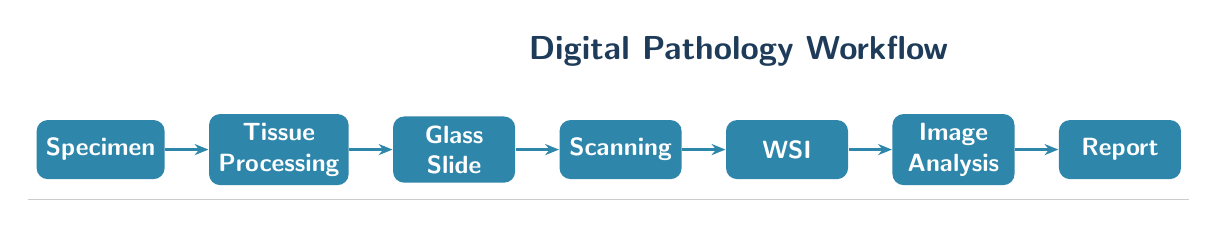
\begin{tikzpicture}[
    node distance = 0.55cm,
    every node/.style = {font=\small\sffamily},
    proc/.style = {
        rectangle,
        rounded corners=4pt,
        fill={rgb,255:red,46;green,134;blue,171},
        text=white,
        minimum width=1.55cm,
        minimum height=0.75cm,
        align=center,
        font=\small\sffamily\bfseries
    },
    arr/.style = {
        -{Stealth[length=5pt,width=4pt]},
        line width=0.8pt,
        color={rgb,255:red,46;green,134;blue,171}
    }
]

%% Title
\node[font=\large\sffamily\bfseries,
      text={rgb,255:red,30;green,60;blue,90}]
    (title) at (0,0) {Digital Pathology Workflow};

%% Nodes placed in a row below the title
\node[proc, below=0.55cm of title, xshift=-8.1cm] (specimen)  {Specimen};
\node[proc, right=0.55cm of specimen]              (tissue)    {Tissue\\Processing};
\node[proc, right=0.55cm of tissue]                (slide)     {Glass\\Slide};
\node[proc, right=0.55cm of slide]                 (scanning)  {Scanning};
\node[proc, right=0.55cm of scanning]              (wsi)       {WSI};
\node[proc, right=0.55cm of wsi]                   (analysis)  {Image\\Analysis};
\node[proc, right=0.55cm of analysis]              (report)    {Report};

%% Arrows
\draw[arr] (specimen) -- (tissue);
\draw[arr] (tissue)   -- (slide);
\draw[arr] (slide)    -- (scanning);
\draw[arr] (scanning) -- (wsi);
\draw[arr] (wsi)      -- (analysis);
\draw[arr] (analysis) -- (report);

%% Subtle baseline rule
\draw[line width=0.4pt, color=gray!40]
    ($(specimen.south west)+(-0.1,-0.25)$) --
    ($(report.south east)+(0.1,-0.25)$);

\end{tikzpicture}

  \caption{Panoramica del flusso di lavoro della patologia digitale. Un campione chirurgico o bioptico viene sottoposto al processamento tissutale standard e sezionato su un vetrino di vetro. Il vetrino colorato viene caricato in uno scanner per vetrini interi, che produce una whole slide image (WSI) gigapixel archiviata su un server di gestione delle immagini. La WSI è quindi disponibile per l'analisi computazionale delle immagini e per la refertazione da parte del patologo, con il referto diagnostico finale trasmesso al team clinico tramite il sistema informativo di laboratorio (LIS).}
  \label{fig:wsi_workflow}
\end{figure}
